%Template on Overleaf made by Andrew K. Schulz, Postdoctoral Researcher in the Haptic Intelligence Department @ Max Planck Institute for Intelligent Systems
%Last updated Nov. 20, 2023
\documentclass[10pt]{article}
\usepackage[utf8]{inputenc}
\usepackage{setspace}
\usepackage{amssymb,verbatim,epsfig}
\usepackage{amsmath,setspace}
\usepackage{multicol}
\usepackage[usenames,dvipsnames]{color}
\addtolength{\topmargin}{-.8in}
\usepackage{wrapfig}
\usepackage{amssymb, amsmath, verbatim, epsfig}
\usepackage{setspace}
\renewcommand {\baselinestretch}{1.}
\topmargin=-1.in
\setlength{\textwidth}{6.5in}
\setlength{\textheight}{9.in}
\setlength{\evensidemargin}{0in}
\setlength{\oddsidemargin}{0in}
\setlength{\topmargin}{-0.4in}
%bib file
\usepackage[comma,sort&compress,super]{natbib}
\setlength{\bibsep}{0pt plus 0.3ex}
\usepackage{graphicx}
\usepackage[font={small}]{caption}
\usepackage[font={small}]{subcaption}
\usepackage{sidecap}
\usepackage{lipsum} % can comment this out, used to insert lipsum text int template
\newcommand{\eq}[1]{Eq.\ (\ref{#1})}
\newcommand{\fig}[1]{{Figure \ref{#1}}}
\newcommand{\tab}[1]{Table \ref{#1}}
\newcommand{\et}{{\it et al}}
\newcommand{\sgn}{\text{sgn}}
\usepackage{xcolor}
\newcommand{\TODO}[1]{{\color{red} {\sf  (TODO #1)}}}
\renewcommand\floatpagefraction{.9}
\renewcommand\topfraction{.9}
\renewcommand\bottomfraction{.9}
\renewcommand\textfraction{.1}
\setcounter{totalnumber}{50}
\setcounter{topnumber}{50}
\setcounter{bottomnumber}{50}

\usepackage{titlesec}
\titleformat{\section}
  {\normalfont\Large\bfseries}{\thesection}{0.2em}{}

%\usepackage[hang,small,bf]{caption}
%\thispagestyle{empty} %no page number
%\addtocounter{page}{-2} %ignore this page when counting
\usepackage{enumitem}


\usepackage{fancyhdr}
\pagestyle{fancy}
\fancyhf{} % clear all header and footer fields
\fancyfoot[R]{\footnotesize \thepage}
\renewcommand\headrule{}
\fancypagestyle{firststyle}
{
	\renewcommand\headrule{}
	\fancyhf{}
}

%This is the template for the Humboldt App, the title page of this document (title, summary, impact) will be cut and pasted into the online form, the rest will be exportable as a PDF and attached. 

\title{\bf Title of Proposal Goes here} %Insert Title of Proposal, this will be pasted into the form
\author{Insert Name Here, Ph.D.\\
\text{\small{Max Planck Institute for Intelligent Systems}}\\
\text{\small{Stuttgart, Germany}}\\
}
\date{}

%%%%
\begin{document}
\maketitle

\noindent \textbf{Keywords:} keyword, keyword, keyword, keyword, keyword %up to five keywords may be included 


\section*{Summary} %brief summary will be pasted into the Humboldt App website
%MAX 2000 characters, in 2023 this character count included spaces. I found no way of putting citations in this. 
%Prompt: Executive summary of the 5-page research proposal. 
\lipsum[1]


\section*{Impact} %impact statement will be posted into the Humboldt App website
%MAX 2000 characters, in 2023 this character count included spaces. I found no way of putting citations into this
%Prompt: What do you think will be the impact of your research on the further development of your own academic profile
\lipsum[1]  
\newpage
%\tableofcontents
%\newpage

%\thispagestyle{firststyle}
%\vspace{0cm}
\pagenumbering{arabic}

%Below is the five pages you have for your research description/research outline for the Humboldt Proposal. Reference list IS INCLUDED in the 5-page count for the proposal. 
\section*{Introduction} %Introduction to the Project

You can include some references you particularly enjoy like this paper\cite{schulz_skin_2022}. % This is the citation format I used throughout. It is possible to change it if you would like. 

\lipsum[1]


\lipsum[2]

\begin{wrapfigure}{r}{0.4\textwidth}
\centering
   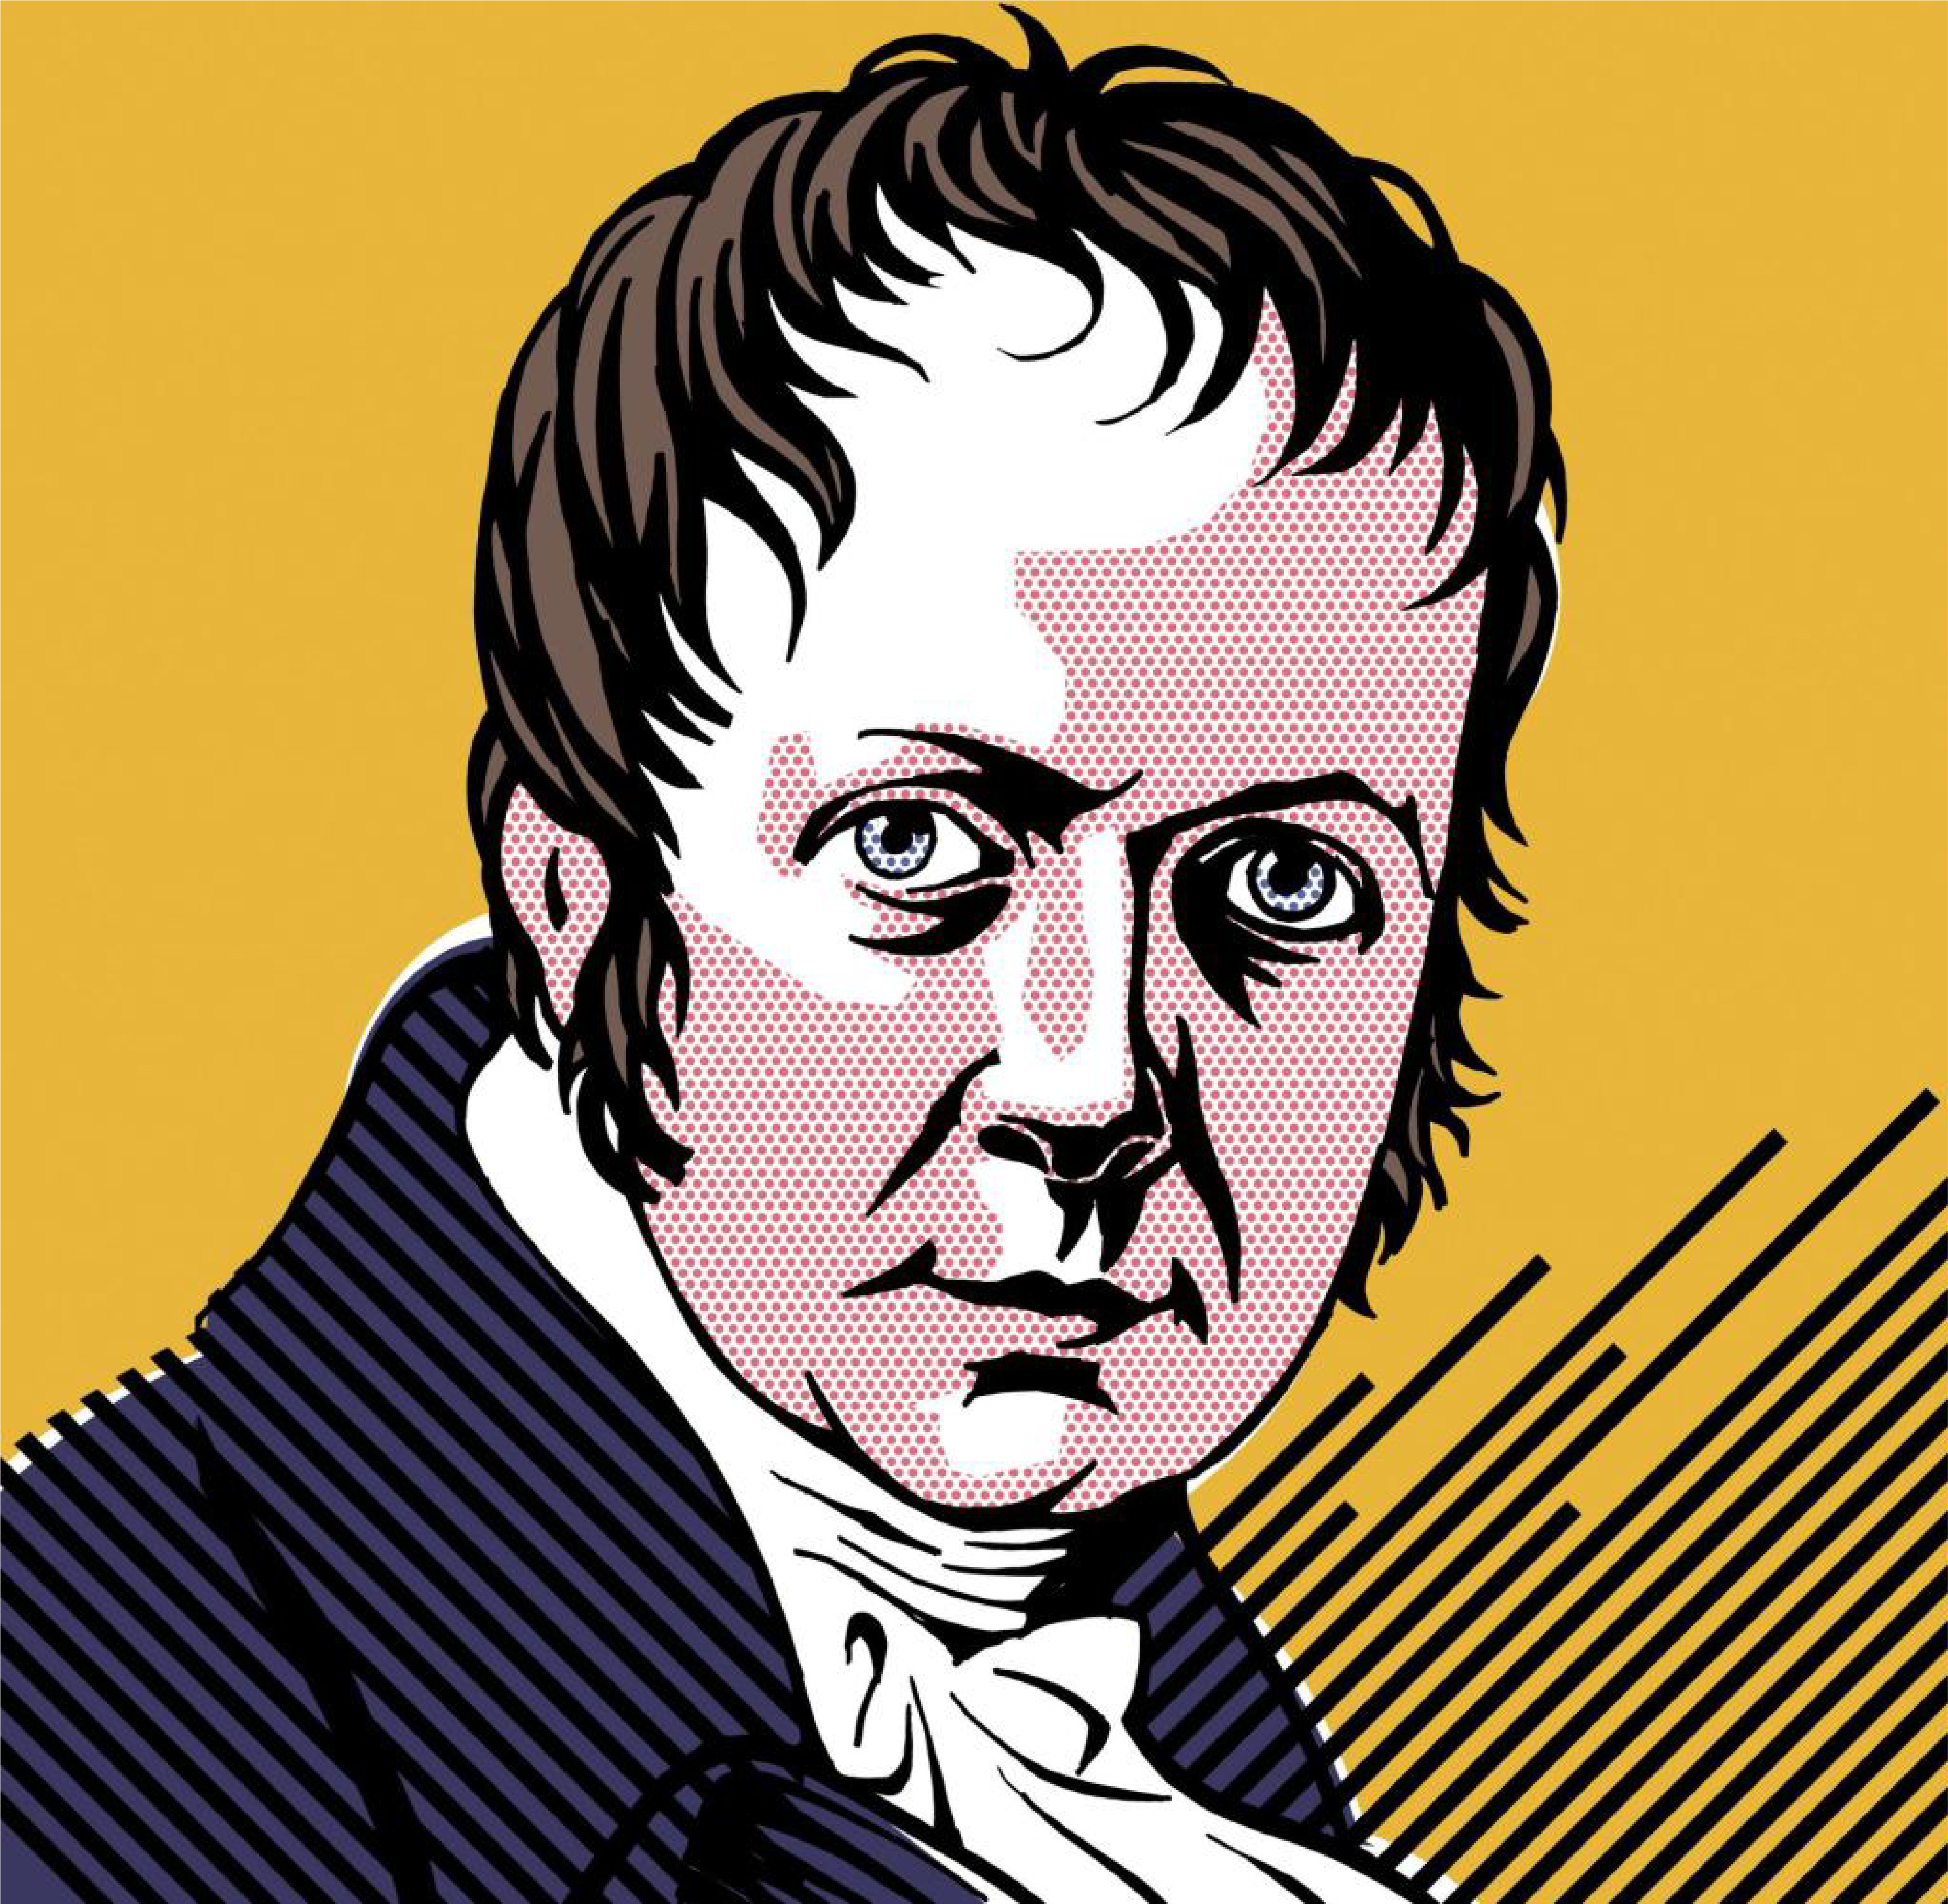
\includegraphics[width=0.4\textwidth]{fig1.png}
   \caption{\label{Fig1}A) This is a figure caption.}
\end{wrapfigure}

\lipsum[1]


\lipsum[2]
\section*{Project Significance} %What significance and background make this project fundable, should also include citations.

\lipsum[1]

\section*{What Questions are to Be Examined?} %This was my formatting choice in 2023, but this is not required. I had two parts of the proposal each with time allotments. 

For this proposal, we are interested in three research questions; each has an associated hypothesis.
\begin{itemize}
	\item {\bf Part 1a: Keyword:} Overall research question?\\
	{\bf Hypothesis:} Testable hypothesis described later in the proposal.
     \vspace{-6pt}
    \item {\bf Part 1b: Keyword:} Overall research question? \\
    {\bf Hypothesis:} Testable hypothesis described later in the proposal. %I added citations to both RQ and Hypotheses when necessary.
    \vspace{-6pt}
	\item {\bf Part 2: Keyword:} Finally research question?\\
	{\bf Hypothesis:} Final testable hypothesis. 
\end{itemize}

In Part 1a, we will examine \ldots \lipsum[1] %here explicitly included in each part what I would do as an executive summary of each question and the collaborators required/needed. 

In Part 1b, we will examine \ldots \lipsum[1] %same as above

In Part 2, we will finalize \ldots 

%I followed this with a brief section about the timeline of the project. 

We will do Part 1a and Part 1b during the first year, performing experiments and the associated theoretical analysis after the experiments are completed. We will proceed with Part 2 after the first year of the project has been completed. We have done preliminary work on each of these areas, and we describe our detailed research plan below, followed by a proposed timeline.

\section*{Proposed Project Methodology} %I broke down the methodology specifically by the research questions and hypothesis. 

\subsection*{Part 1a: Materials Methodology}
\lipsum[1]

\subsection*{Part 1b: Mechanics Methodology}



\lipsum[1]

\subsection*{Part 2: Bio-Inspiration Methodology}
\lipsum[1]

%\section*{Timeline}
%In Year 1 XX. 
\vspace{-12pt}
\bibliographystyle{abbrv} %This is the bibliography style I used. I do not believe there are specific instructions in 2023 on which bib file type to use. If more room is needed you can make the bibliography tiny.
\small \bibliography{refsbib}
\newpage

\end{document}
